date : 5 december 2023

\subsubsection*{Ontwerp Parameters van Voedingen}

\begin{enumerate}[label=--]
  \item \textbf{Ingangsspanning:} \\
    Beschrijving van de vereiste ingangsspanning voor de voeding.

  \item \textbf{Uitgangsspanning:} \\
    Beschrijving van de gewenste uitgangsspanning van de voeding.

  \item \textbf{Dissipatie en Rendement:} \\
    Specificatie van de dissipatie en het rendement van de voeding.

  \item \textbf{Ruis:} \\
    Beschrijving van de gewenste niveaus van ruis in de voeding.

  \item \textbf{Inschakelverschijnselen:} \\
    Verklaring van de verschijnselen die optreden bij het inschakelen van de voeding.

  \item \textbf{Uitschakelverschijnselen:} \\
    Verklaring van de verschijnselen die optreden bij het uitschakelen van de voeding.
\end{enumerate}

\subsubsection{decibel}
\begin{figure}[H]
\centering
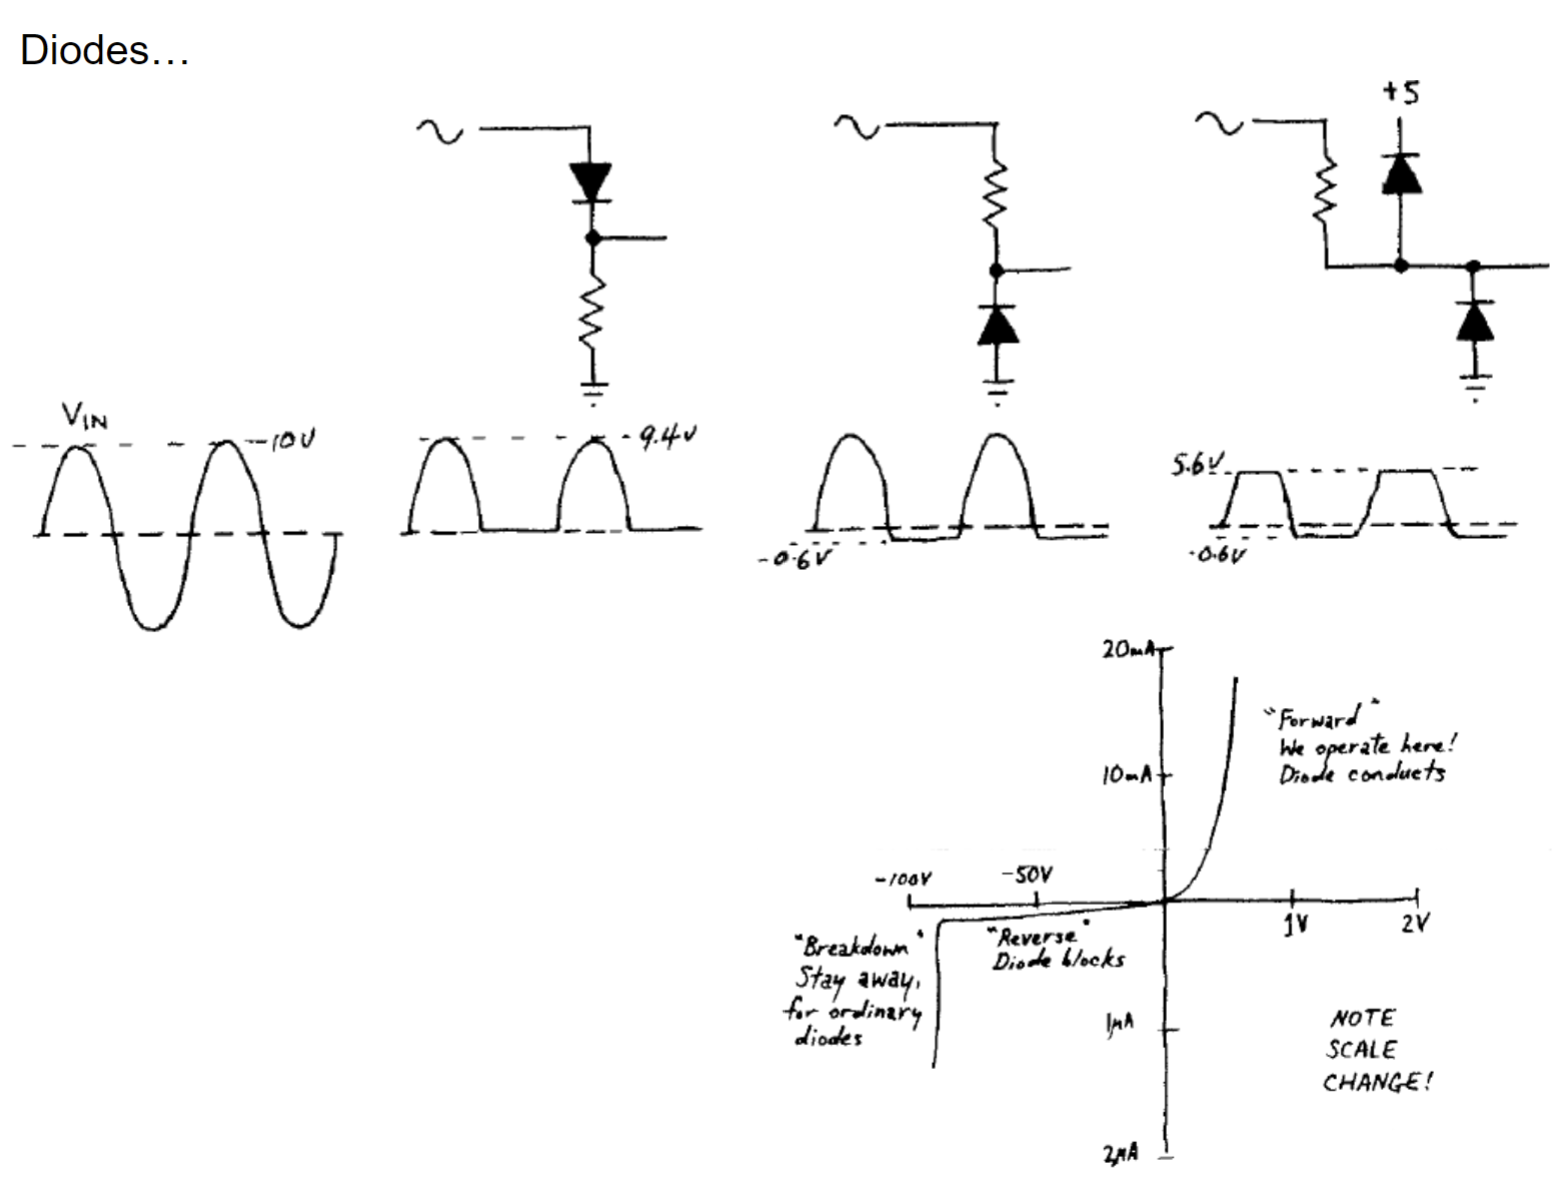
\includegraphics[scale=0.5]{Diode.png}
\end{figure}

\subsubsection*{Verschil tussen een Normale Diode en een Zener-diode}

Een \textbf{normale diode} en een \textbf{Zener-diode} zijn beide halfgeleiderapparaten die stroom in één richting laten stromen. Het belangrijkste verschil tussen deze twee typen diodes ligt in hun gedrag bij omgekeerde polarisatie.\\

Een normale diode laat stroom in slechts één richting toe en blokkeert stroom in de omgekeerde richting. Wanneer de diode in de omgekeerde richting wordt gepolariseerd boven een bepaalde spanning, zal er een punt komen waarop de diode zal doorslaan en stroom gaat geleiden in omgekeerde richting. Dit wordt het \textit{omgekeerde knelpunt} genoemd en moet worden vermeden in normale toepassingen.\\

Een Zener-diode is ontworpen om bewust te werken in de omgekeerde doorslagregio. De belangrijkste eigenschap van een Zener-diode is het handhaven van een vrijwel constante spanning over zijn terminals, zelfs wanneer deze in omgekeerde polarisatie is aangesloten en het omgekeerde knelpunt heeft bereikt. Deze constante omgekeerde spanning wordt de \textit{Zener-spanning} genoemd.\\

In toepassingen wordt een Zener-diode vaak gebruikt als spanningsregelaar, waarbij het stabiele Zener-spanningsniveau wordt gebruikt om een constante uitgangsspanning te handhaven.

\subsubsection*{DC/DC Converters}
\begin{figure}[H]
    \centering
    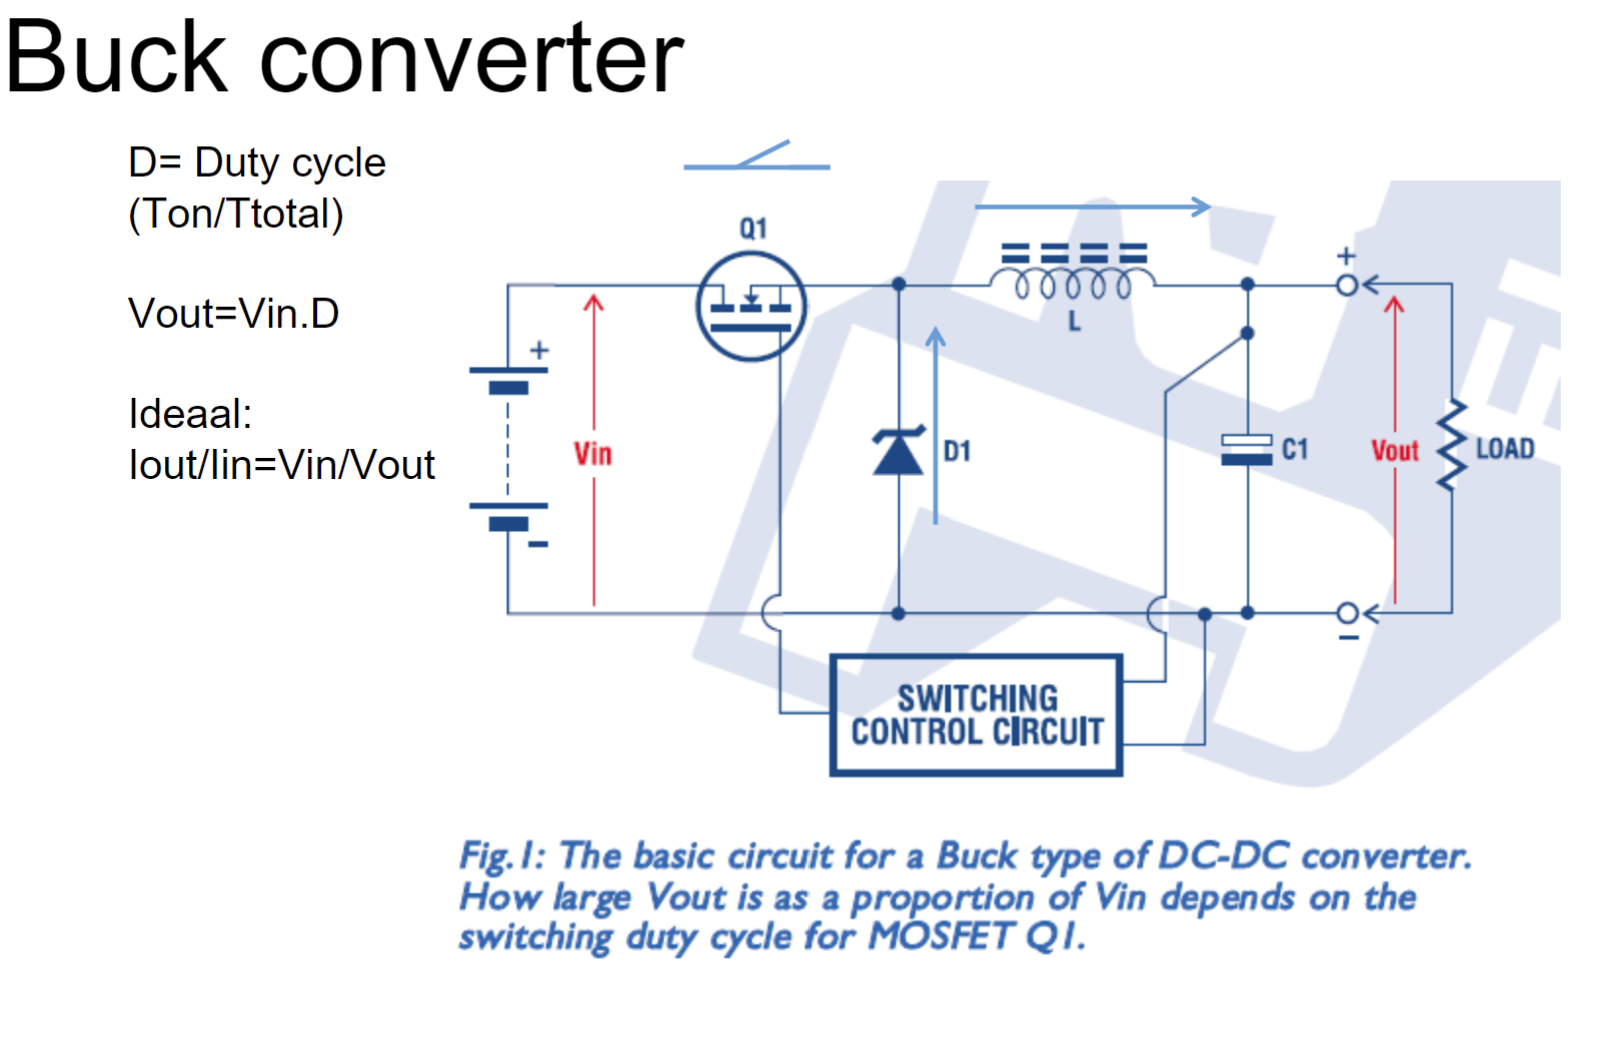
\includegraphics[scale=0.5]{Buck.png}
    \caption*{ non isolated spannings verlager}
    \end{figure}
\begin{figure}[H]
    \centering
    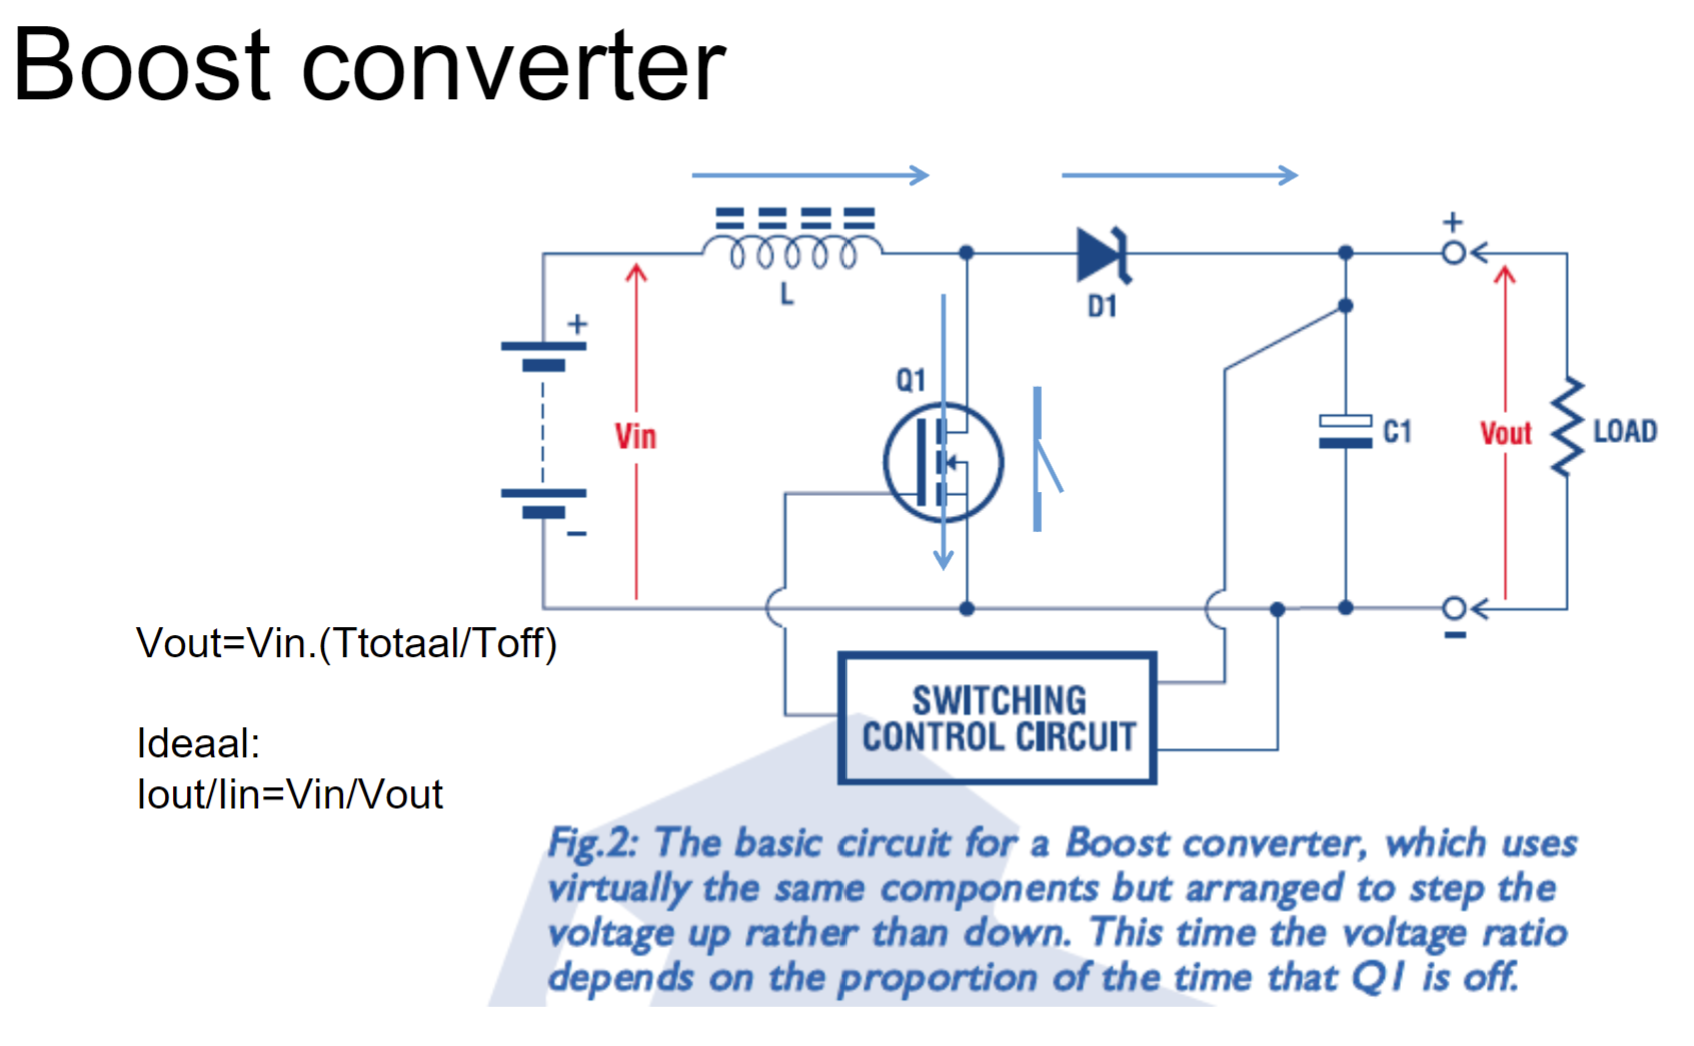
\includegraphics[scale=0.5]{boost.png}
    \caption*{ non isolated spannings verhoger}
    \end{figure}
\begin{figure}[H]
    \centering
    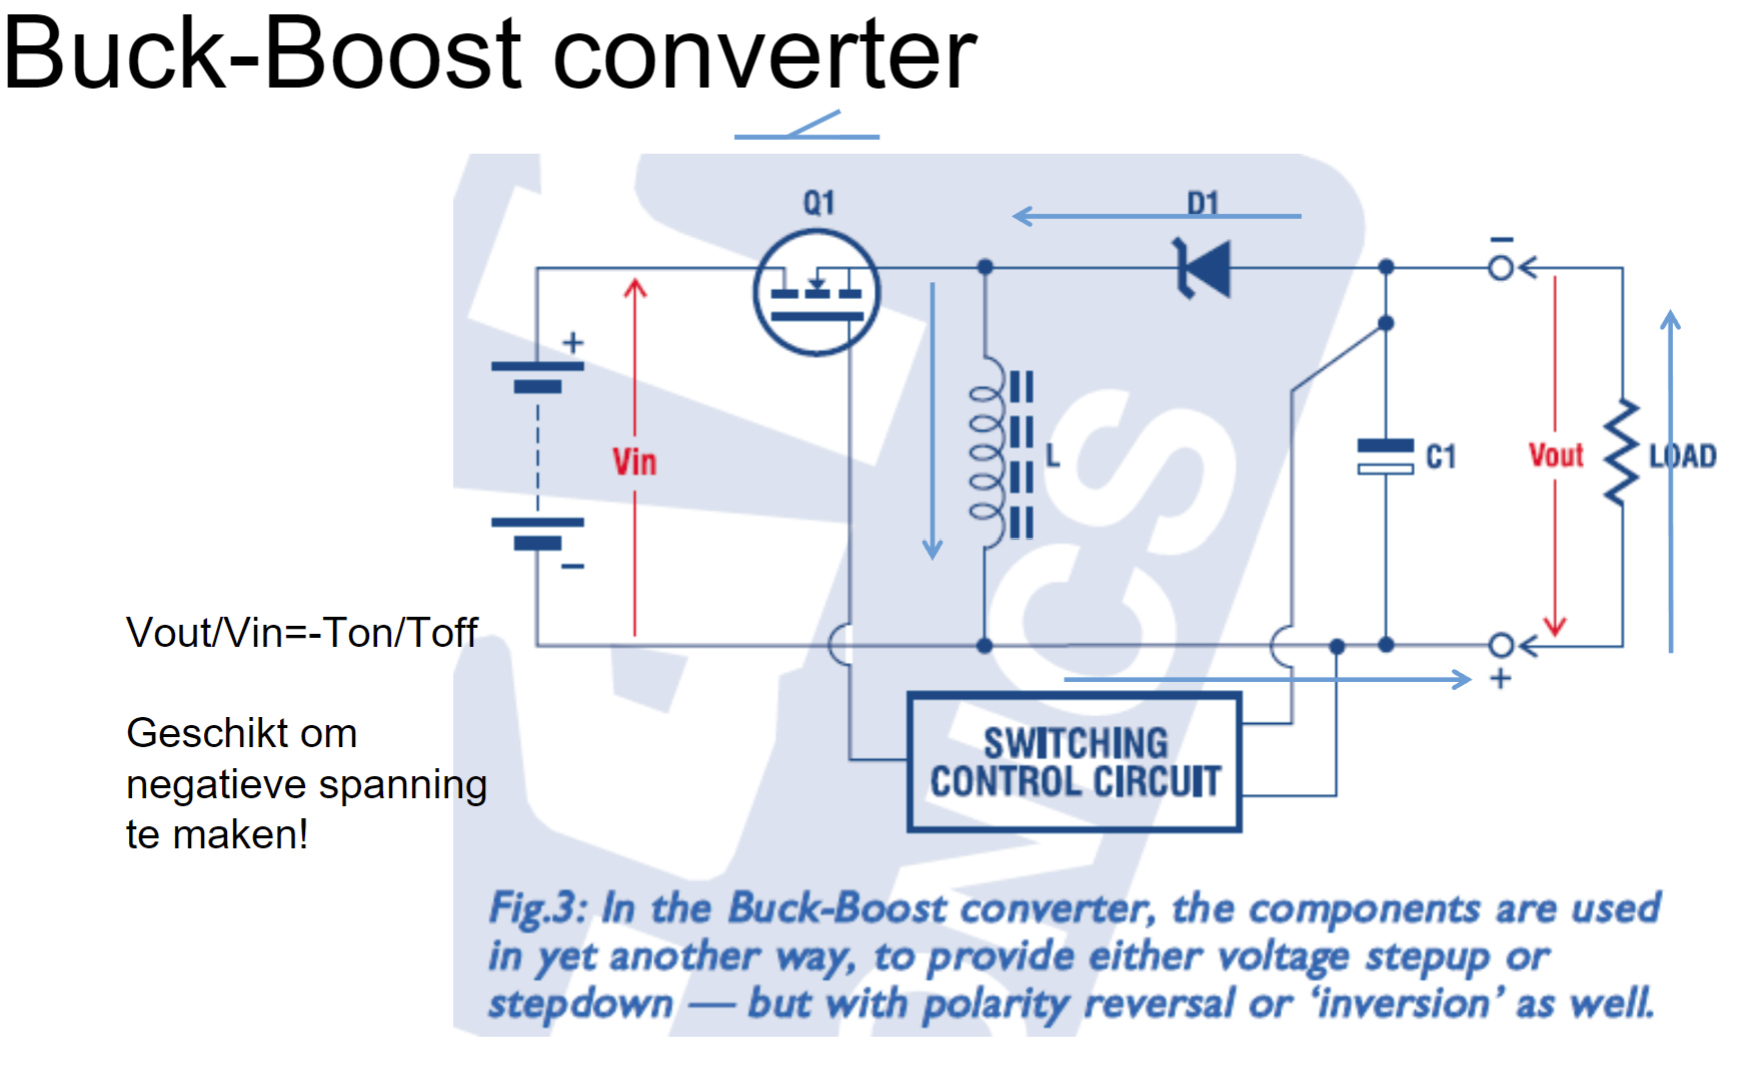
\includegraphics[scale=0.5]{buck-boost.png}
    \caption*{ non isolated spannings verhoger en verlager}
    \end{figure}
\begin{figure}[H]
    \centering
    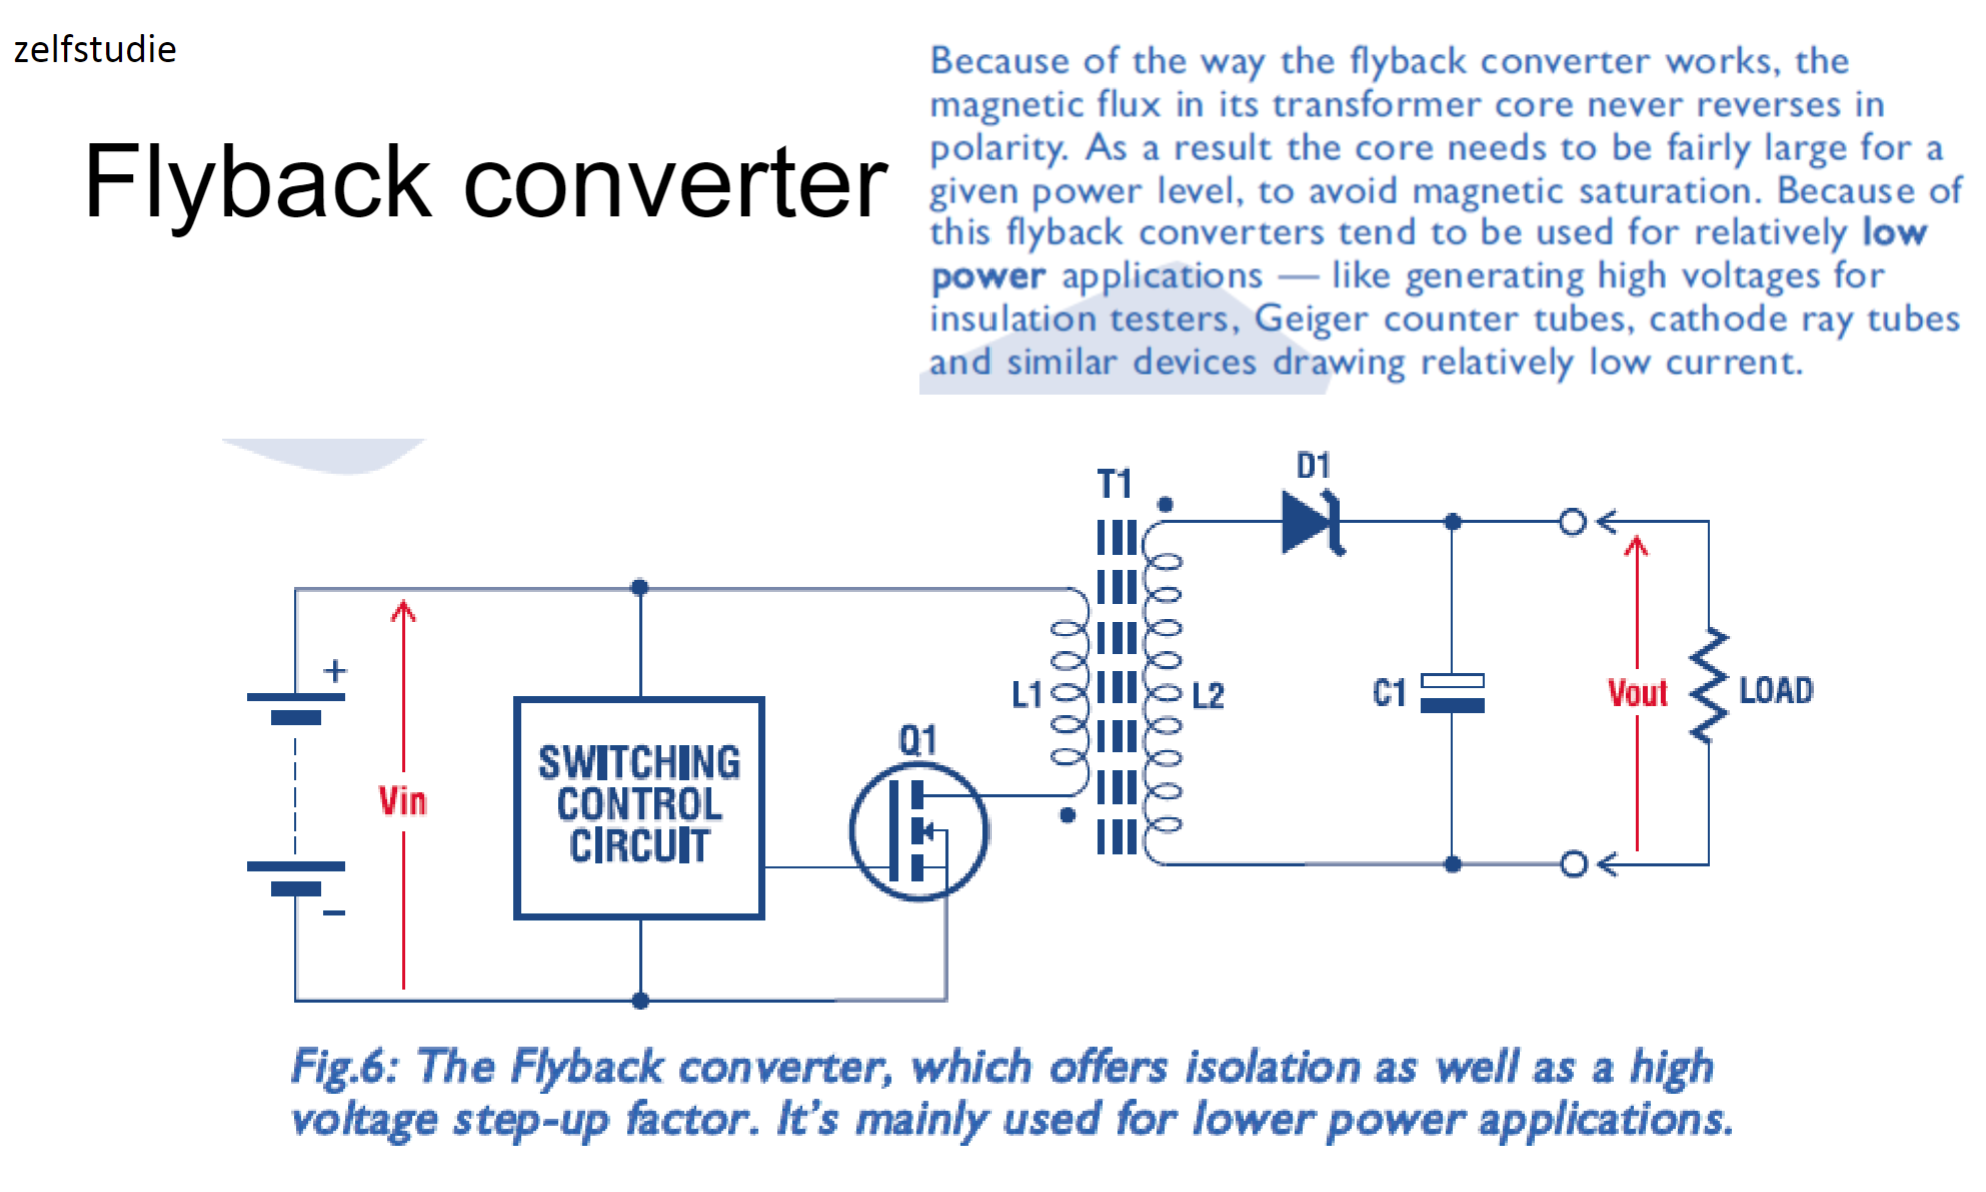
\includegraphics[scale=0.5]{flyback.png}
    \caption*{ Isolated converter Flyback}
    \end{figure}
\begin{figure}[H]
    \centering
    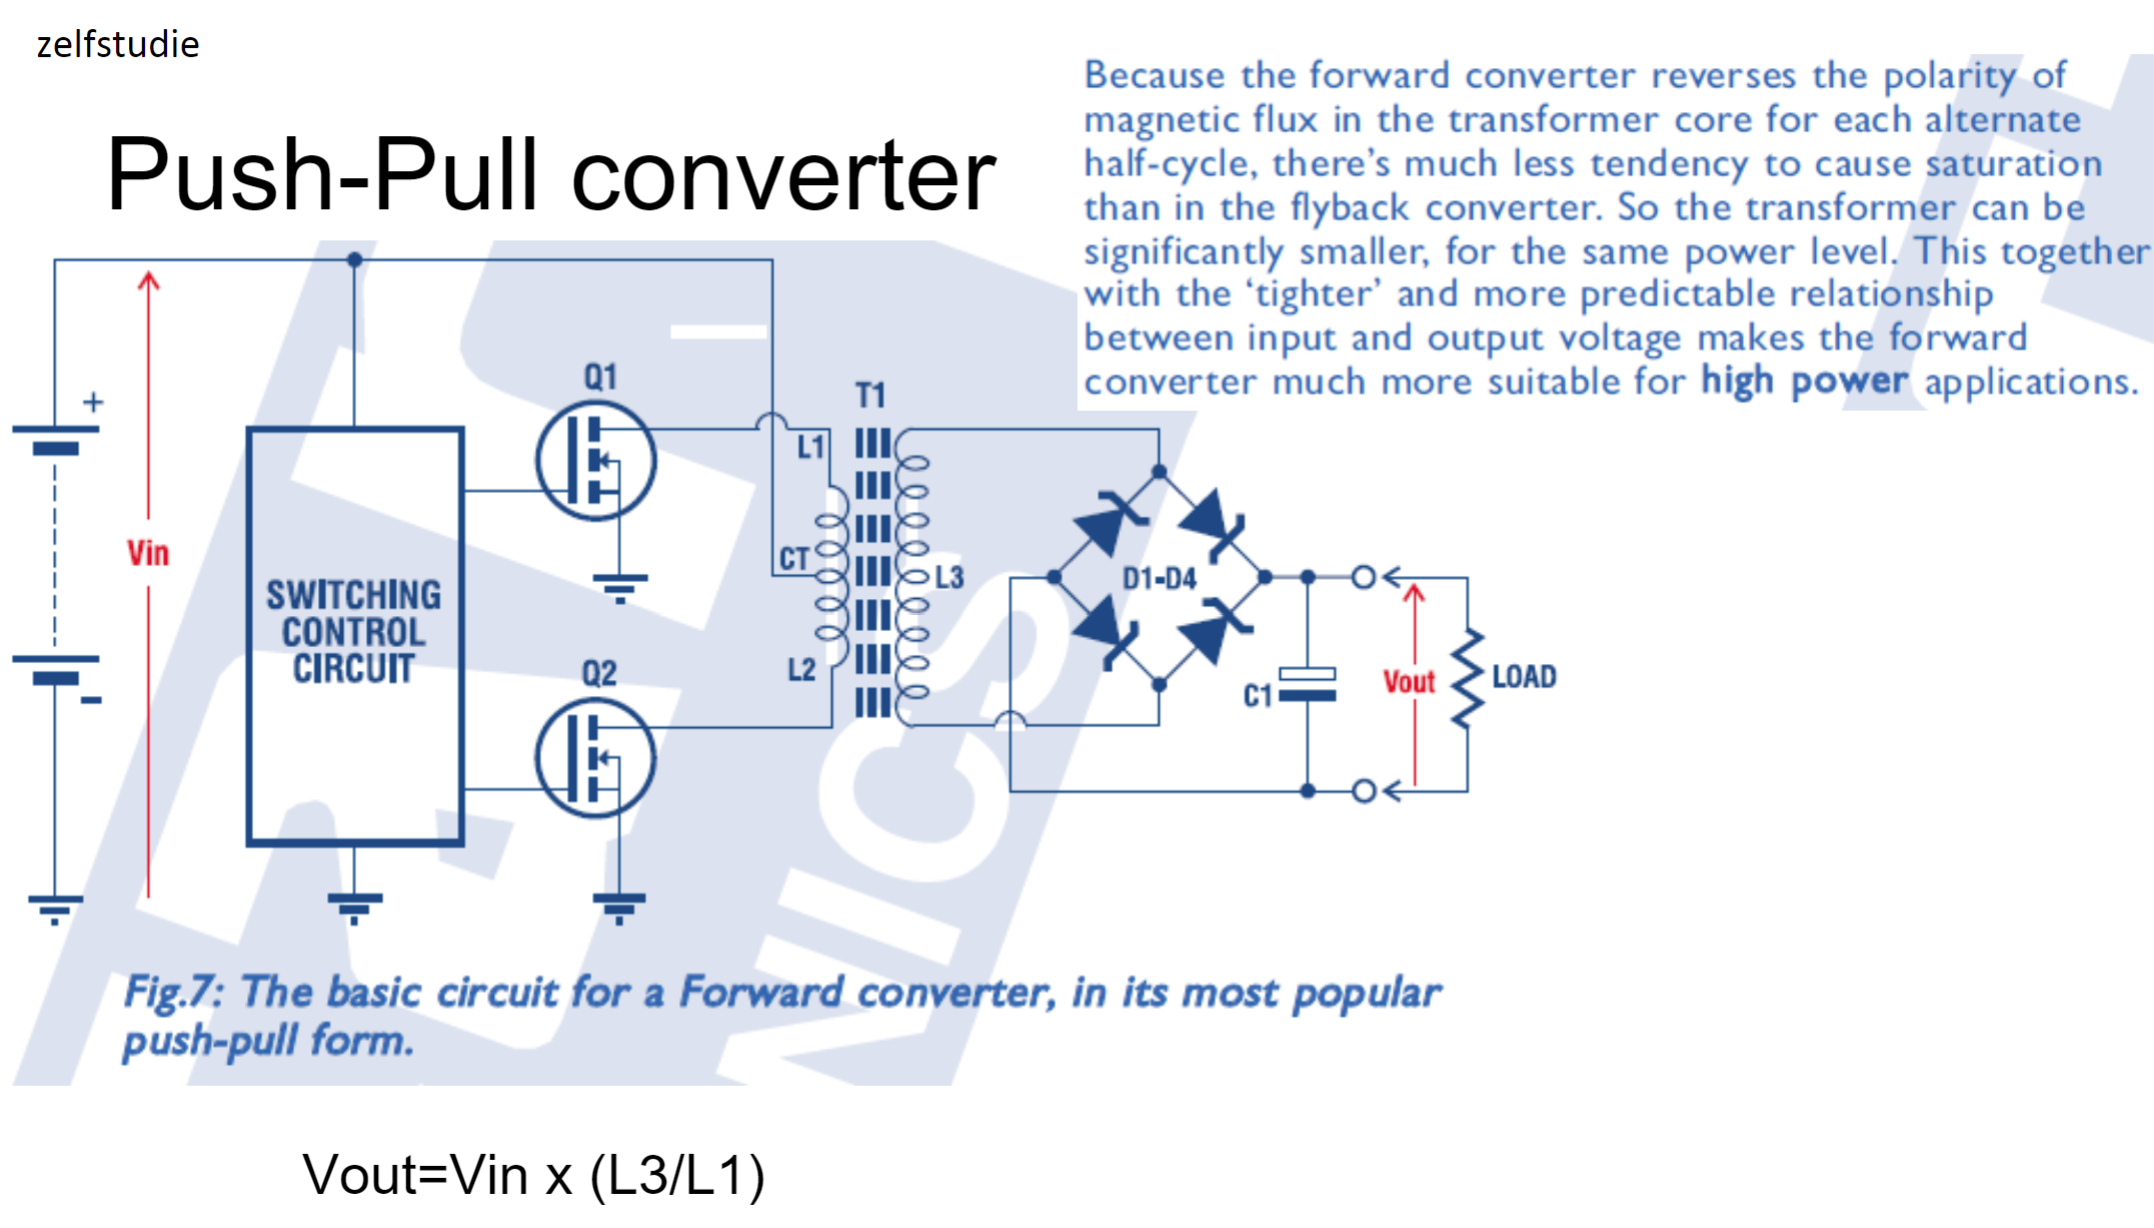
\includegraphics[scale=0.5]{push-pull.png}
    \caption*{ Isolated converter push pull}
    \end{figure}


Verbeteringen
\begin{itemize}
    \item Synchronous rectification
    \item Overal waar een diode staat -> geschakelde mosfet
    \item Clock sync
\end{itemize}
Hogere frequenties
\begin{itemize}
    \item Nieuwe materialen!
    \item Maakt kleinere converters mogelijk....
\end{itemize}

\vspace{1cm}
Switcher of LDO??\\
Switcher:
\begin{itemize}
    \item Betere efficiëntie
    \item Blijft koel
    \item Kan van zo ongeveer alle Uin alle Uout maken
    \item Zeer nauwkeurig PCB plan
\end{itemize}
LDO:
\begin{itemize}
    \item Geen storende frequenties door schakelen
    \item Single chip Solutions (op de Cap na!)
    \item Goedkoop
    \item Rendement is relatief laag (Udrop out bepaald minimum)
\end{itemize}
